% Foliensatz: "AFu-Kurs nach DJ4UF" von DK0TU, Amateurfunkgruppe der TU Berlin
% Lizenz: CC BY-NC-SA 3.0 de (http://creativecommons.org/licenses/by-nc-sa/3.0/de/)
% Autor: Felix Baum DB4UM <baum@campus.tu-berlin.de>
% Korrekturen: Lars Weiler <dc4lw@darc.de>

\documentclass[aspectratio=169]{beamer}

\usepackage[ngerman]{babel} % deutsche Worttrennung etc.
\usepackage[utf8]{inputenc} % UTF8 Text

\usepackage[super, comma, numbers, square, sort]{natbib}

\usepackage{hyperref}       % Hyperref Package für bessere Referenzen (todo)
\hypersetup{
	colorlinks=false,       %   false: boxed links; true: colored links
    %linkcolor=white,       %   color of internal links (change box color with linkbordercolor)
    citecolor=red,          %   color of links to bibliography
    filecolor=white,        %   color of file links
    urlcolor=blue           %   color of external links
}

\usepackage{multirow}
\usepackage{wasysym}  % Math Symbols like \permil
%\usepackage{colortbl}
%\usepackage{subscript}
%\usepackage{caption}
%\usepackage{setspace}
%\usepackage{xcolor}        % benutze CodeListe

% Footnote
%\usepackage{hanging}
%
%\setbeamertemplate{footnote}{%
%  \hangpara{2em}{1}%
%  \makebox[2em][l]{\insertfootnotemark}\footnotesize\insertfootnotetext\par%
%}


%\usepackage{pgf}
%\usepackage{tikz}
%\usetikzlibrary{arrows,automata}
%\usetikzlibrary{positioning}
%
%\tikzset{
%    state/.style={
%           rectangle,
%           rounded corners,
%           draw=black, very thick,
%           minimum height=2em,
%           minimum width=2pt,
%           inner sep=2pt,
%           text centered,
%           },
%}

%\usepackage{listings}
%\lstset{basicstyle=\small, numberstyle=\tiny, extendedchars=true, numbers=left, numbersep=5pt}
%\lstset{showtabs=false, showspaces=false, showstringspaces=false}
%%\lstset{backgroundcolor=\color{white!75!lightgray}, , frame=single}
%%\lstset{backgroundcolor=\color{white}}
%%\lstset{backgroundcolor=none}
%\lstset{keywordstyle=\color{blue!50!gray},  identifierstyle=\color{black}}
%\lstset{commentstyle=\color{green!50!gray}, stringstyle=\color{red!50!gray}}
%\lstset{language=C, fontadjust=true, tabsize=2, breaklines=true}
%\lstset{backgroundcolor=\color{white!75!lightgray}, caption=\lstname, frame=single}
%\lstset{emphstyle=\color{black}\fbox}
%
%% Keine "Listing:"-Caption
%\captionsetup{labelformat=empty,labelsep=none}
%
%% für mathematische Umgebungen
%\usepackage{amsmath,amsfonts,amssymb}
%
%\lstdefinestyle{Bash}{
%language=Bash,
%frame=single,
%rulecolor=\color{black},
%backgroundcolor=\color{gray!50},
%keywordstyle=\color{black},
%identifierstyle=,
%commentstyle=\color{black},
%stringstyle=\color{magenta!65!white},
%showstringspaces=false,
%basicstyle=\footnotesize\ttfamily\color{black},
%numbers=none,
%breaklines=true,
%captionpos=b
%}

%\usepackage{listings}
%
%\lstdefinestyle{basic}{
%    captionpos=t,%
%    basicstyle=\footnotesize\ttfamily,%
%    numberstyle=\tiny,%
%    numbers=left,%
%    stepnumber=1,%
%    frame=single,%
%    showspaces=false,%
%    showstringspaces=false,%
%    showtabs=false,%
%    %
%    keywordstyle=\color{blue},%
%    identifierstyle=,%
%    commentstyle=\color{gray},%
%    stringstyle=\color{magenta}%
%}



% fließende Boxen haben keinen Abstand
%\fboxsep0mm

% inkludiere Creative Commons Helper
%%%%%%%%%%%%%%%%%%%%%%%%%%%%%%%%%%%%%%%%%%%%%%%%%%%%%%%%%%%%%%%%
%% ccBeamer 0.1, 2007-07-02                                   %%
%% Written by Sebastian Pipping <webmaster@hartwork.org>      %%
%% ---------------------------------------------------------- %%
%% Licensed under Creative Commons Attribution-ShareAlike 3.0 %%
%% http://creativecommons.org/licenses/by-sa/3.0/             %%
%%%%%%%%%%%%%%%%%%%%%%%%%%%%%%%%%%%%%%%%%%%%%%%%%%%%%%%%%%%%%%%%


%% Images
\newcommand{\CcImageBy}[1]{%
	
\includegraphics[scale=#1]{texdata/creative_commons/cc_by_30.pdf}%
}
\newcommand{\CcImageCc}[1]{%
	
\includegraphics[scale=#1]{texdata/creative_commons/cc_cc_30.pdf}%
}
\newcommand{\CcImageDevNations}[1]{%
	
\includegraphics[scale=#1]{texdata/creative_commons/cc_dev_nations_30.pdf}%
}
\newcommand{\CcImageNc}[1]{%
	
\includegraphics[scale=#1]{texdata/creative_commons/cc_nc_30.pdf}%
}
\newcommand{\CcImageNd}[1]{%
	
\includegraphics[scale=#1]{texdata/creative_commons/cc_nd_30.pdf}%
}
\newcommand{\CcImagePd}[1]{%
	
\includegraphics[scale=#1]{texdata/creative_commons/cc_pd_30.pdf}%
}
\newcommand{\CcImageSa}[1]{%
	
\includegraphics[scale=#1]{texdata/creative_commons/cc_sa_30.pdf}%
}
\newcommand{\CcImageSampling}[1]{%
	
\includegraphics[scale=#1]{texdata/creative_commons/cc_sampling_30.pdf}%
}
\newcommand{\CcImageSamplingPlus}[1]{%
	
\includegraphics[scale=#1]{texdata/creative_commons/cc_sampling_plus_30.pdf}%
}


%% Groups
\newcommand{\CcGroupBy}[2]{% zoom, gap
	\CcImageCc{#1}\hspace*{#2}\CcImageBy{#1}%
}
\newcommand{\CcGroupByNc}[2]{% zoom, gap
	\CcImageCc{#1}\hspace*{#2}\CcImageBy{#1}\hspace*{#2}\CcImageNc{#1}%
}
\newcommand{\CcGroupByNcNd}[2]{% zoom, gap
	\CcImageCc{#1}\hspace*{#2}\CcImageBy{#1}\hspace*{#2}\CcImageNc{#1}\hspace*{#2}\CcImageNd{#1}%
}
\newcommand{\CcGroupByNcSa}[2]{% zoom, gap
	\CcImageCc{#1}\hspace*{#2}\CcImageBy{#1}\hspace*{#2}\CcImageNc{#1}\hspace*{#2}\CcImageSa{#1}%
}
\newcommand{\CcGroupByNd}[2]{% zoom, gap
	\CcImageCc{#1}\hspace*{#2}\CcImageBy{#1}\hspace*{#2}\CcImageNd{#1}%
}
\newcommand{\CcGroupBySa}[2]{% zoom, gap
	\CcImageCc{#1}\hspace*{#2}\CcImageBy{#1}\hspace*{#2}\CcImageSa{#1}%
}
\newcommand{\CcGroupDevNations}[2]{% zoom, gap
	\CcImageCc{#1}\hspace*{#2}\CcImageDevNations{#1}%
}
\newcommand{\CcGroupNcSampling}[2]{% zoom, gap
	\CcImageCc{#1}\hspace*{#2}\CcImageNc{#1}\hspace*{#2}\CcImageSampling{#1}%
}
\newcommand{\CcGroupPd}[1]{% zoom
	\CcImagePd{#1}%
}
\newcommand{\CcGroupSampling}[1]{% zoom
	\CcImageSampling{#1}%
}
\newcommand{\CcGroupSamplingPlus}[1]{% zoom
	\CcImageSamplingPlus{#1}%
}


%% Text
\newcommand{\CcLongnameBy}{Attribution}
\newcommand{\CcLongnameByNc}{Attribution-NonCommercial}
\newcommand{\CcLongnameByNcNd}{Attribution-NoDerivs}
\newcommand{\CcLongnameByNcSa}{Attribution-NonCommercial-ShareAlike}
\newcommand{\CcLongnameByNd}{Attribution-NoDerivs}
\newcommand{\CcLongnameBySa}{Attribution-ShareAlike}

\newcommand{\CcNote}[1]{% longname
	This work is licensed under the \textit{Creative Commons #1 3.0 License}.%
}


% generelles Thema auswählen
\usetheme{Goettingen} %Berlin spart ohne Sidebar allerdings angenehm Platz
% AnnArbor | Antibes | Bergen | Berkeley | Berlin | Boadilla | boxes | CambridgeUS | Copenhagen | Darmstadt | default | Dresden | Frankfurt | Goettingen | Hannover | Ilmenau | JuanLesPins | Luebeck | Madrid | Malmoe | Marburg | Montpellier | PaloAlto | Pittsburgh | Rochester | Singapore | Szeged | Warsaw

% Farben wählen
\usecolortheme{beetle}
% beaver | beetle | crane | default | dolphin | dove | fly | lily | orchid | rose | seagull | seahorse | sidebartab | structure | whale | wolverine

% Setze alle Farben auf Grau und Weiß
%\definecolor{craneorange}{RGB}{64,64,64}
%\definecolor{craneblue}{RGB}{255,255,255}

% Schriftart wählen
\usefonttheme{default}
% default | professionalfonts | serif | structurebold | structureitalicserif | structuresmallcapsserif

% Innere Themen(Kopf-, Fuß-, Sidebar usw)
%\useinnertheme{default}
\useinnertheme{circles}
% default | inmargin | rectangles | rounded | circles

% Äußere Themen (Anordnung der inneren, grenzen der Folien etc.)
\useoutertheme{infolines}
% default | infolines | miniframes | shadow | sidebar | smoothbars | smoothtree | split | tree

% Deaktiviere Navigations-Symbole ({} -> leer)
\setbeamertemplate{navigation symbols}{}
%\setbeamertemplate{navigation symbols}{\large \ifnum \insertframenumber <10 0\fi\insertframenumber/\inserttotalframenumber\vspace*{0.2ex}}

% Zeige ein Hintergrundbild
\setbeamertemplate{background canvas}{
        \hspace*{-2.0cm}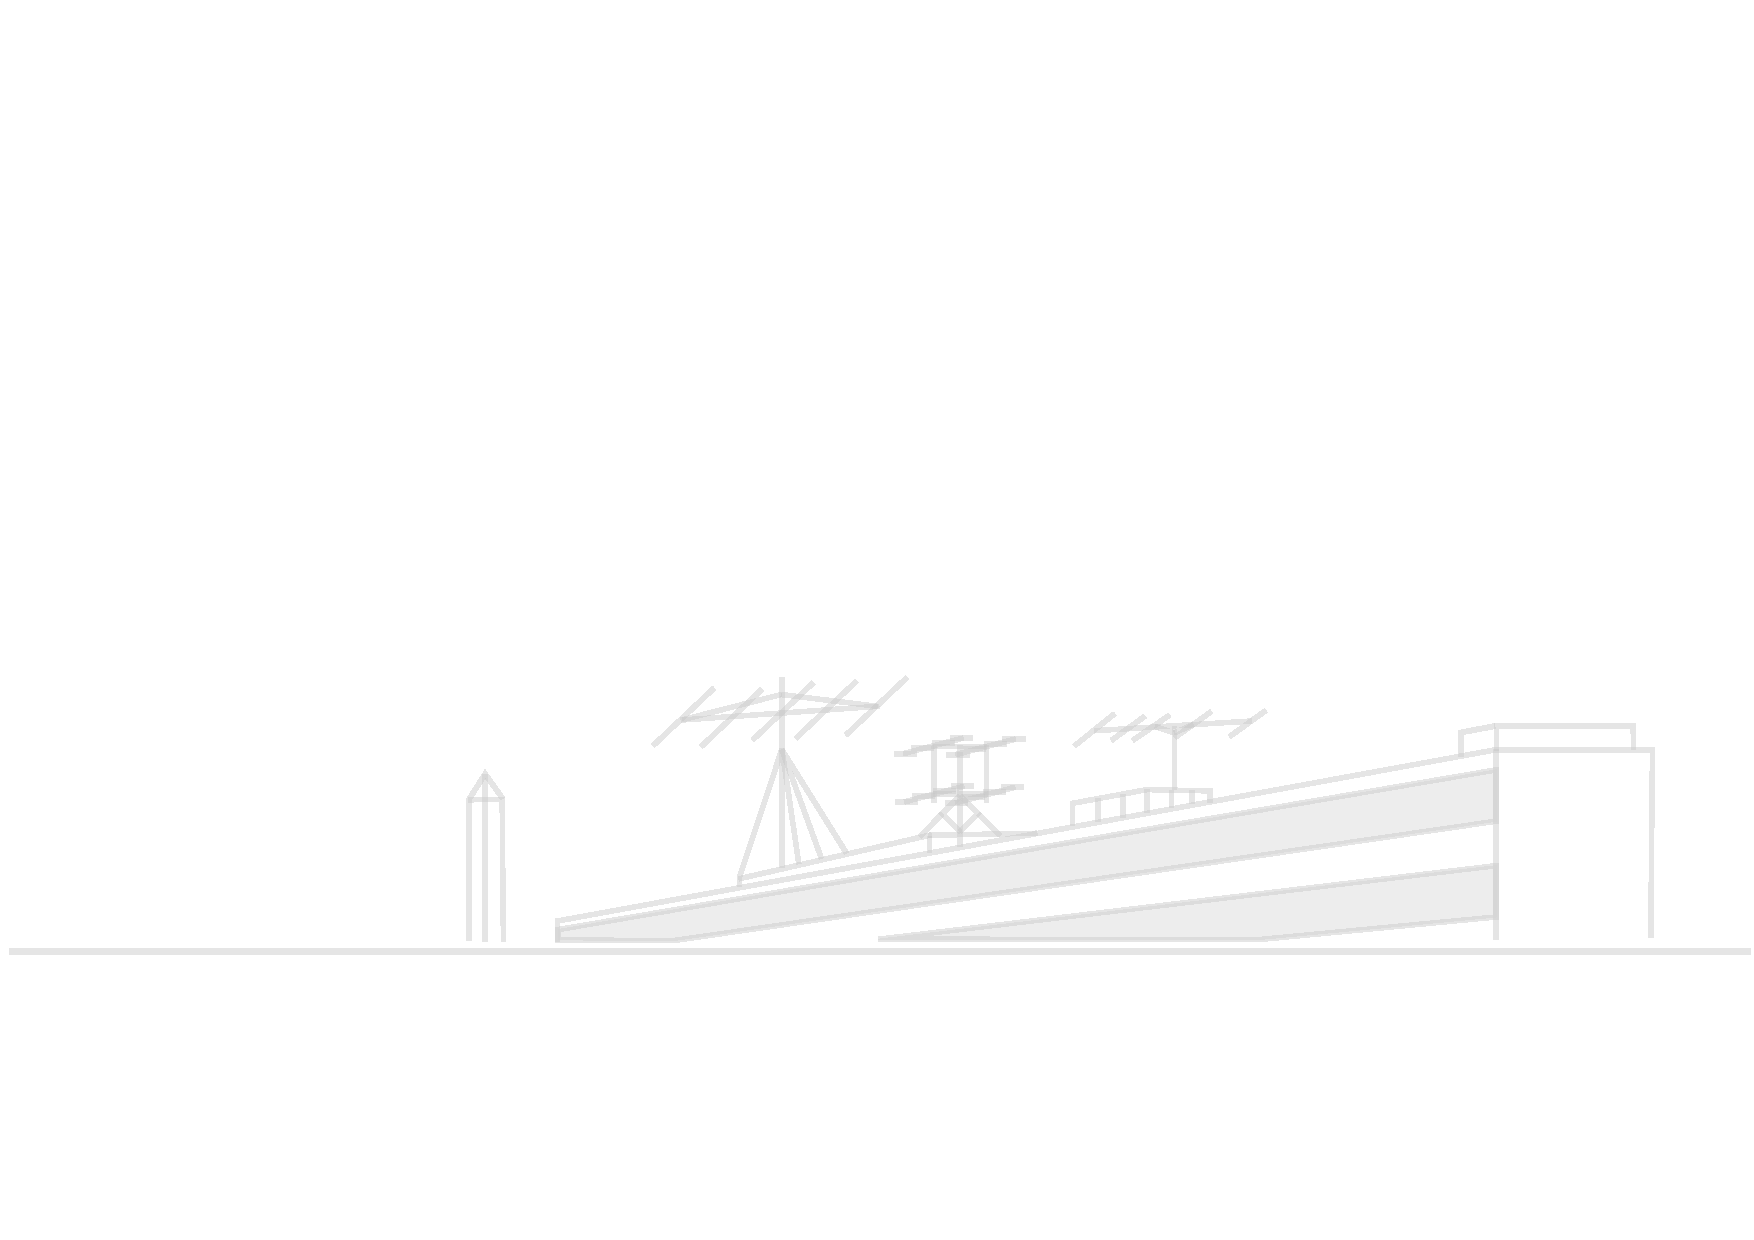
\includegraphics[width=17.8cm]{texdata/dk0tu_rooftop_background.pdf}
}

% Foliennummer einfügen
\setbeamertemplate{footline}[frame number]
%\setbeamertemplate{footline}{}

% Ändere das Zeichen vor jedem item
%\setbeamertemplate{itemize item}{\color{craneorange}$\blacktriangleright$}
%\setbeamertemplate{itemize subitem}{\color{craneorange}$\triangleright$}
%\setbeamertemplate{itemize subsubitem}{\color{craneorange}$\blacktriangleright$}

% Ändert die Blöcke 
\setbeamertemplate{blocks}[rounded][shadow=true]
% default | rounded [shadow=true|false]

%
% Eigene Kommandos
%

% Hack to get natbib and beamer working together. "The beamer user guide suggests
% that only the manual bibliography entry approach is supported"
% on some system it works out of the box, sometimes you need the hack :-(
% so check it --dl7bst
\ifdefined\newblock
    \relax
\else
    \newcommand{\newblock}{}
\fi

% \includedia command to generate png out of a dia file
% NEEDS installed dia and pdflatex option --shell-escape
\newcommand{\includedia}[1]{
    \immediate\write18{/usr/bin/dia #1.dia -e #1_diatmp.png -t png}
}

% RICHIG GROSSER FONT!
\newfont{\bigfont}{cmr10 at 144pt}
\newfont{\smallfont}{cmr10 at 8pt}

% Römische Ziffern
\makeatletter
\newcommand{\rmnum}[1]{\romannumeral #1}
\newcommand{\Rmnum}[1]{\expandafter\@slowromancap\romannumeral #1@}
\makeatother

% Schwarze Überschrift
%\setbeamercolor{frametitle}{fg=black}
%\setbeamercolor{title}{fg=black}

% Item- und Box-Farben
\definecolor{deepBlue}{HTML}{000066}
\setbeamercolor{itemize item}{fg=deepBlue}
\setbeamercolor{itemize subitem}{fg=deepBlue}
\setbeamercolor{description item}{fg=deepBlue}
\setbeamercolor{block title}{fg=deepBlue!100, bg=blue!15}
\setbeamercolor{block body}{fg=black, bg=blue!5}
\setbeamercolor{block title alerted}{fg=deepBlue, bg=red!75}
\setbeamercolor{block body alerted}{fg=black, bg=red!15}
\setbeamercolor*{block title example}{fg=blue!50, bg=blue!10}
\setbeamercolor*{block body example}{fg= blue, bg=blue!5}

%\setbeamercolor{section in head/foot}{parent=palette primary}
%\setbeamercolor{subsection in head/foot}{parent=palette secondary}
%\setbeamercolor{sidebar}{fg=darkblue,bg=yellow!90!orange}
%\setbeamercolor{title in sidebar}{fg=darkblue}
%\setbeamercolor{author in sidebar}{fg=darkblue}
%\setbeamercolor{section in sidebar}{fg=darkblue!10!black}
%\setbeamercolor{subsection in sidebar}{fg=darkblue!50!black}

% Titlepage Infos
\title{AFu-Kurs nach DJ4UF}
\author[DKØTU]{DKØTU\\ \footnotesize{Amateurfunkgruppe der TU Berlin}}
\institute[DKØTU]{\url{http://www.dk0tu.de} }

% PDF-Eigenschaften
\subject{DK0TU-Amateurfunkkurs nach DJ4UF}
\keywords{Amateurfunk Kurs HAM Radio Course CC-BY-NC-SA OpenSource TU Berlin DK0TU}

\subtitle{Technik E 17: \\
          Messtechnik \\[2em]}
\date{Stand 21.12.2015}
 \begin{document}

\begin{frame}
    \titlepage
    \vfill
    \begin{center}
        \ccbyncsaeu\\
        {\tiny This work is licensed under the \em{Creative Commons Attribution-NonCommercial-ShareAlike 3.0 License}.}\\[0.5ex]
         \tiny Amateurfunkgruppe der Technische Universität Berlin (AfuTUB), DKØTU
         %\includegraphics[scale=0.5]{img/DK0TU_Logo.pdf}
    \end{center}
\end{frame}


%fixme Referenzen/Fußnoten-Systematik vereinheitlichen

\section*{Einleitung}

\begin{frame}
    \frametitle{Messgeräte}
    \begin{itemize}
		\item Was kann alles beim Funken gemessen werden?
    \end{itemize}
\end{frame}
  
\section*{Analog}

\begin{frame}
    \frametitle{Drehspulenmessgerät (Antik)}
	\begin{minipage}{0.3\textwidth}
	    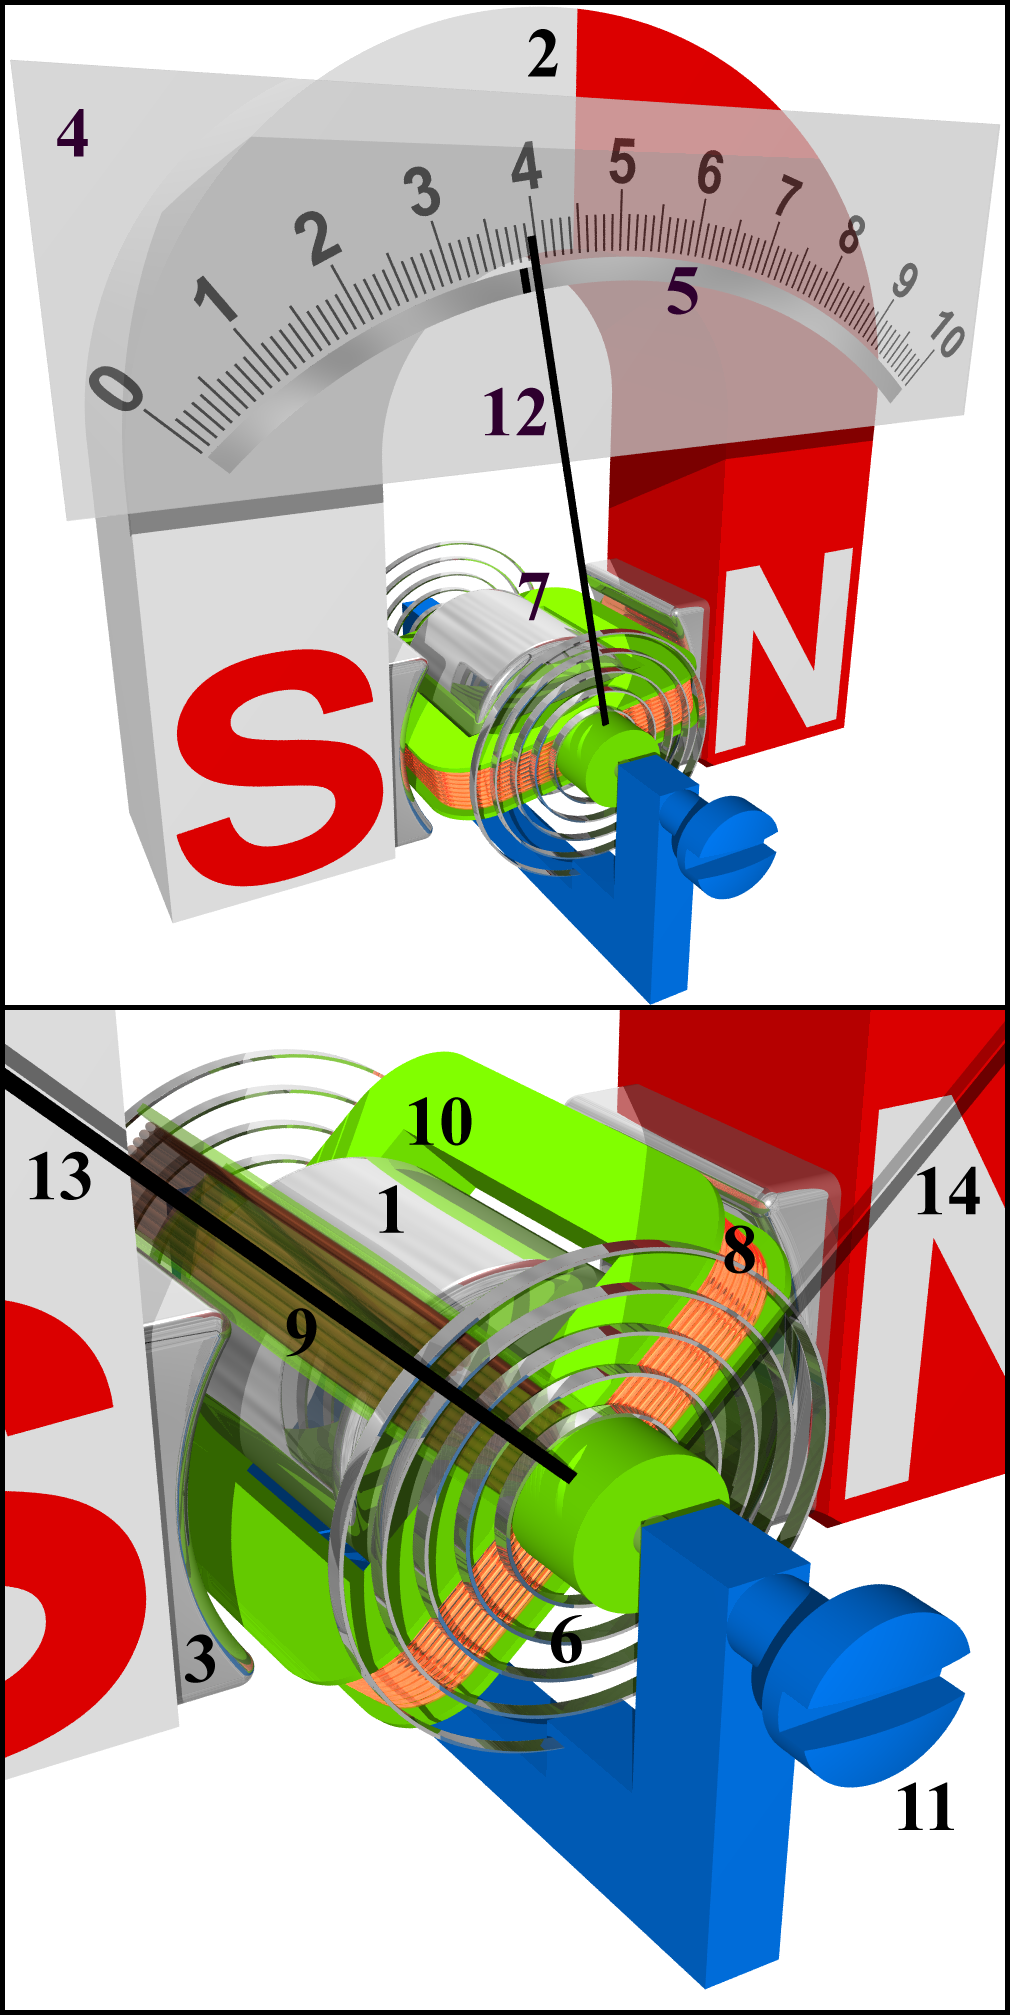
\includegraphics[width=.95\textwidth,height=.8\textheight,keepaspectratio]{e17/drehspulenMess.png}\\
	\end{minipage}
	        \footnote{\tiny \url{https://commons.wikimedia.org/wiki/File:Moving_coil_instrument_principle.png}}
		%\hspace{0.5cm}
	\begin{minipage}{0.65\textwidth}
	\begin{enumerate} \footnotesize
		\item  Weicheisenkern der Drehspule
		\item  Permanentmagnet
		\item  Polschuh zur Bündelung des Magnetfeldes
		\item  Skala
		\item  Hilfsspiegel zur genauen Ablesung
		\item  Rückstellfeder
		\item  Drehspule
		\item  Drehspule in Nulllage
		\item  Drehspule bei Maximalausschlag
		\item  Joch der Spule
		\item  Stellschraube für Nullpunkteinstellung
		\item  Zeiger
		\item  Zeiger in Nulllage
		\item  Zeiger bei Maximalausschlag
	\end{enumerate}
	\end{minipage}
\end{frame}

\begin{frame}
    \frametitle{Prüfungsfrage}
    \begin{center}
        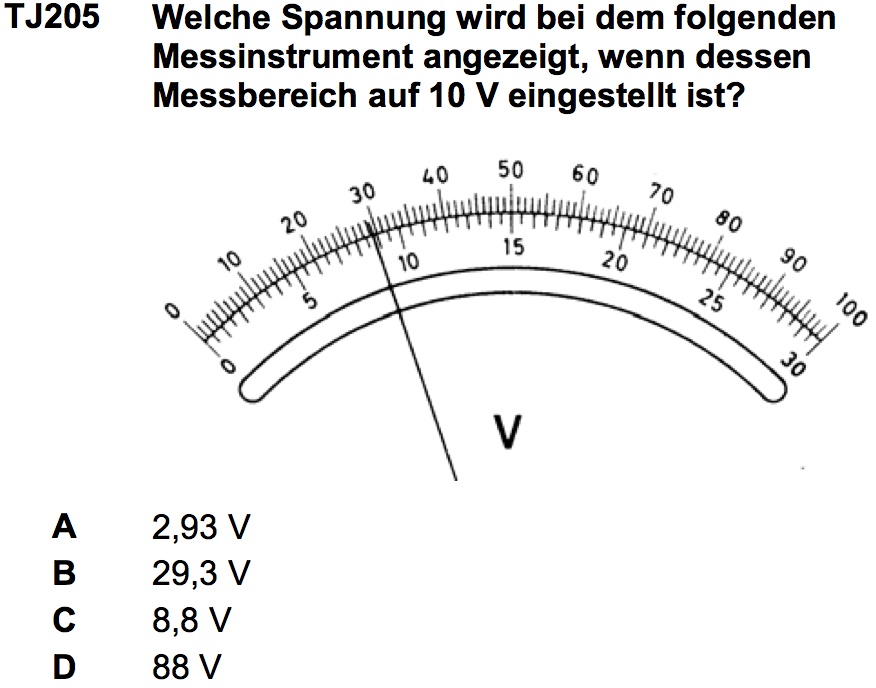
\includegraphics[width=.95\textwidth,height=.8\textheight,keepaspectratio]{e17/messbereich.png}
        \footnote{\tiny Fragenkatalog BundesNetzAgentur Klasse E}
	\end{center}
\end{frame}

\section*{Digital}

\begin{frame}
    \frametitle{Digitales Multimeter}
    \begin{center}
        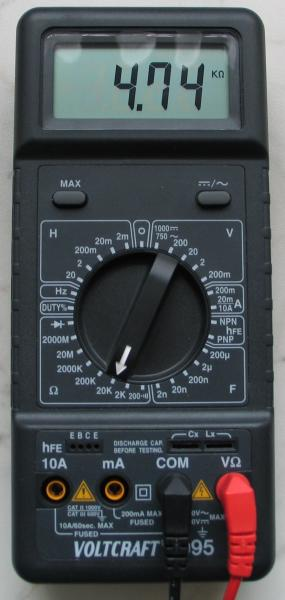
\includegraphics[width=.35\textwidth,height=.9\textheight,keepaspectratio]{e17/digitalmultimeter.jpg}
	\end{center}
\end{frame}

\begin{frame}
    \frametitle{Was wo anschließen?}
	\begin{minipage}{0.4\textwidth}
        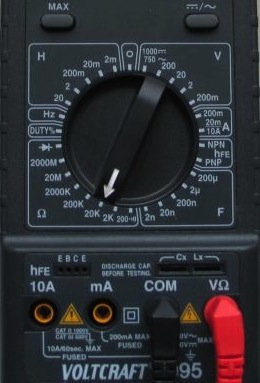
\includegraphics[width=1\textwidth,height=.9\textheight,keepaspectratio]{e17/digitalmultimeterMess.jpg}
	\end{minipage}
	\begin{minipage}{0.55\textwidth}
	\begin{itemize}
		\item Was kann alles gemessen werden?
		\item Wo anschließen zum Strom messen?
		\item Wo anschließen zum Spannung messen?
		\item Welcher Messbereich?
	\end{itemize}
	\end{minipage}
\end{frame}

\begin{frame}
    \frametitle{Wie sollte gemessen werden?}
        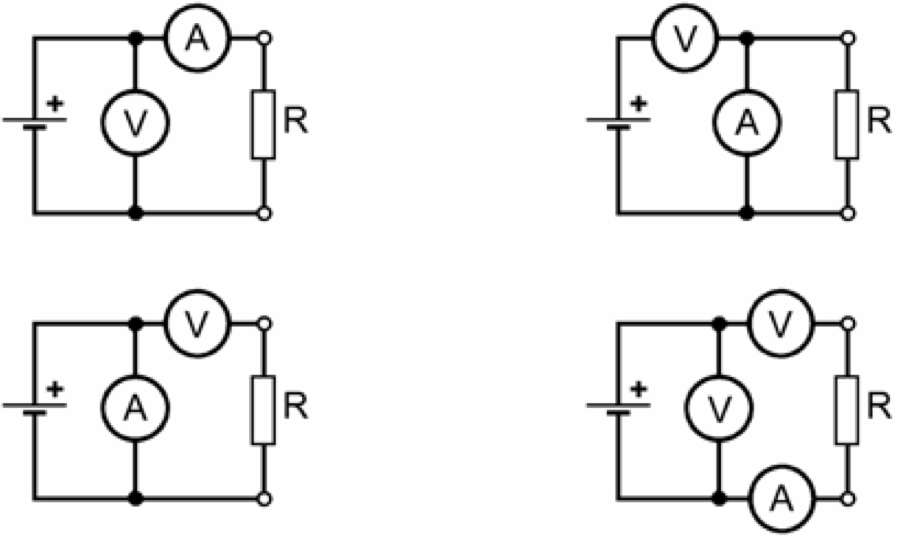
\includegraphics[width=1\textwidth,height=.8\textheight,keepaspectratio]{e17/stromSpannung.png}
        \footnote{\tiny Fragenkatalog BundesNetzAgentur Klasse E}
\end{frame}

\begin{frame}
    \frametitle{Messfehler}
    \begin{center}
      \begin{tabular}{ccc}
	Nullpunktabweichung & Empfindlichkeitsabweichung & Linearitätsabweichung
      \end{tabular}
      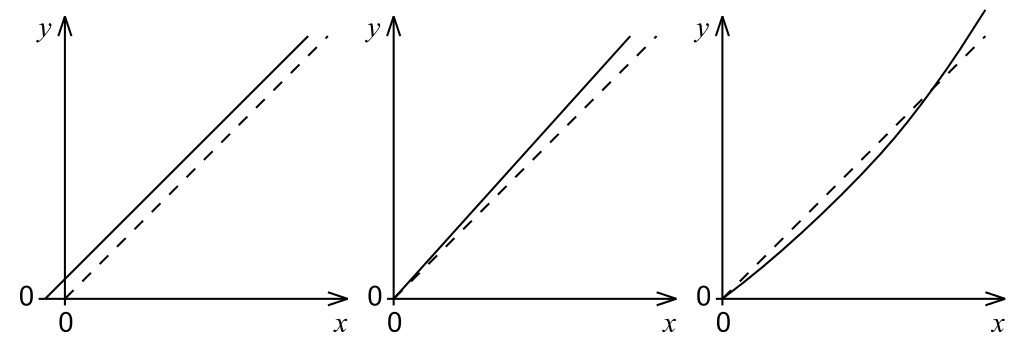
\includegraphics[width=1\textwidth,height=.6\textheight]{e17/werMisstMisst.png}
      \footnote{\tiny \url{https://commons.wikimedia.org/wiki/File:AMT_Fehler.svg}}
    \end{center}
\end{frame}

\begin{frame}
    \frametitle{Prüfungsfrage}
      \begin{tabular}{l||p{.8\textwidth}}\hline
	\textbf{TJ102} & \textbf{Die Auflösung eines Messinstrumentes entspricht\ldots} \\  \hline\hline
         A  & der Genauigkeit des Instrumentes in Bezug auf den tatsächlichen Wert. \\ \hline
         B & der Genauigkeit des Instrumentes. \\ \hline
         C \only<2>\checkmark & der kleinsten Einteilung der Anzeige. \\\hline
         D & dem Vollausschlag der Instrumentenanzeige. \\\hline
    \end{tabular}
\end{frame}

\section*{Oszilloskop}

\begin{frame}
    \frametitle{Oszilloskop}
    \begin{center}
        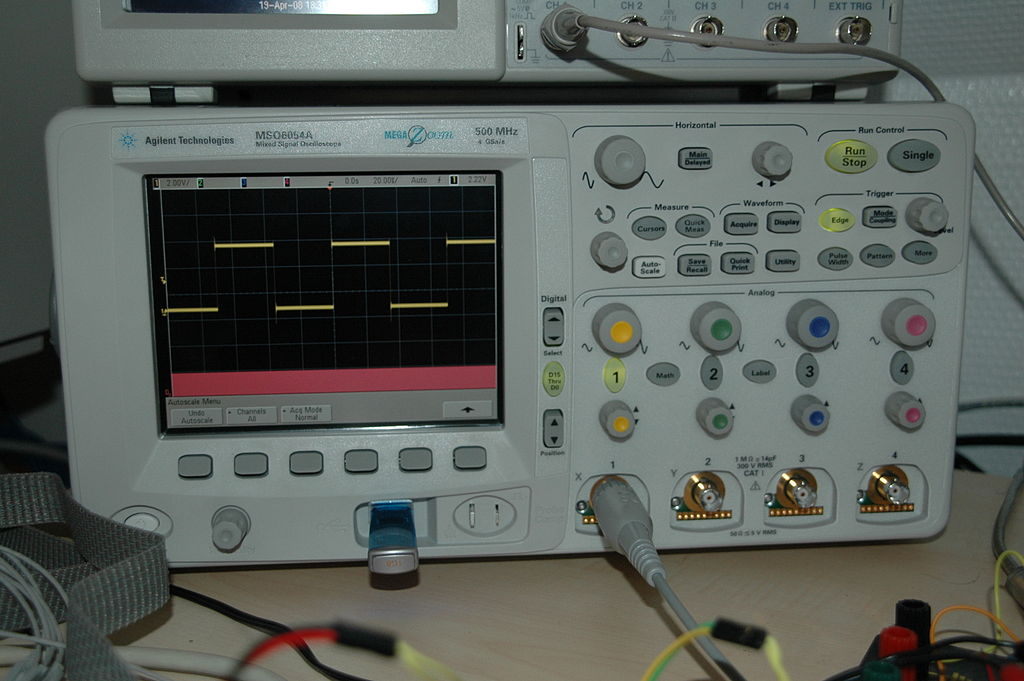
\includegraphics[width=1\textwidth,height=.8\textheight,keepaspectratio]{e17/osziModern.jpg}
        \footnote{\tiny \url{https://commons.wikimedia.org/wiki/File:Modernes_Speicheroszilloskop.jpg}}
	\end{center}
\end{frame}

\begin{frame}
    \frametitle{Oszilloskop}
    \begin{center}
        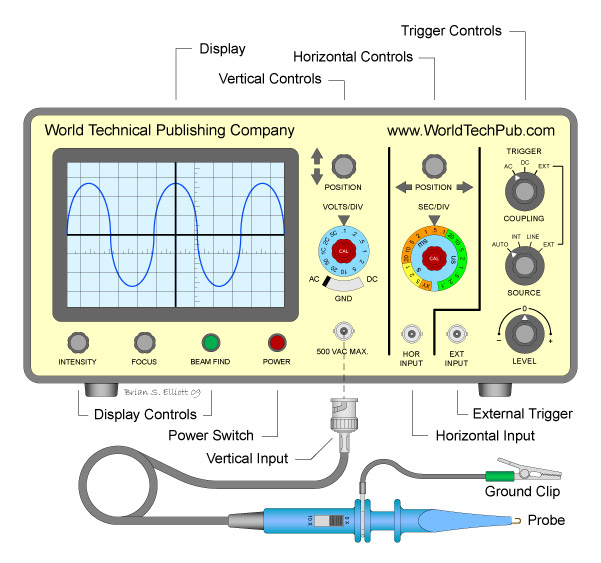
\includegraphics[width=.8\textwidth,height=.8\textheight,keepaspectratio]{e17/WTPCOscilloscopeBeschreiben.jpg}
        \footnote{\tiny \url{https://en.wikipedia.org/wiki/File:WTPC_Oscilloscope-1.jpg}}
	\end{center}
\end{frame}

\begin{frame}
    \frametitle{Oszilloskop -- Ablesen}
    \begin{center}
        $100mV / Div$ und $0.1ms / Div$\\
        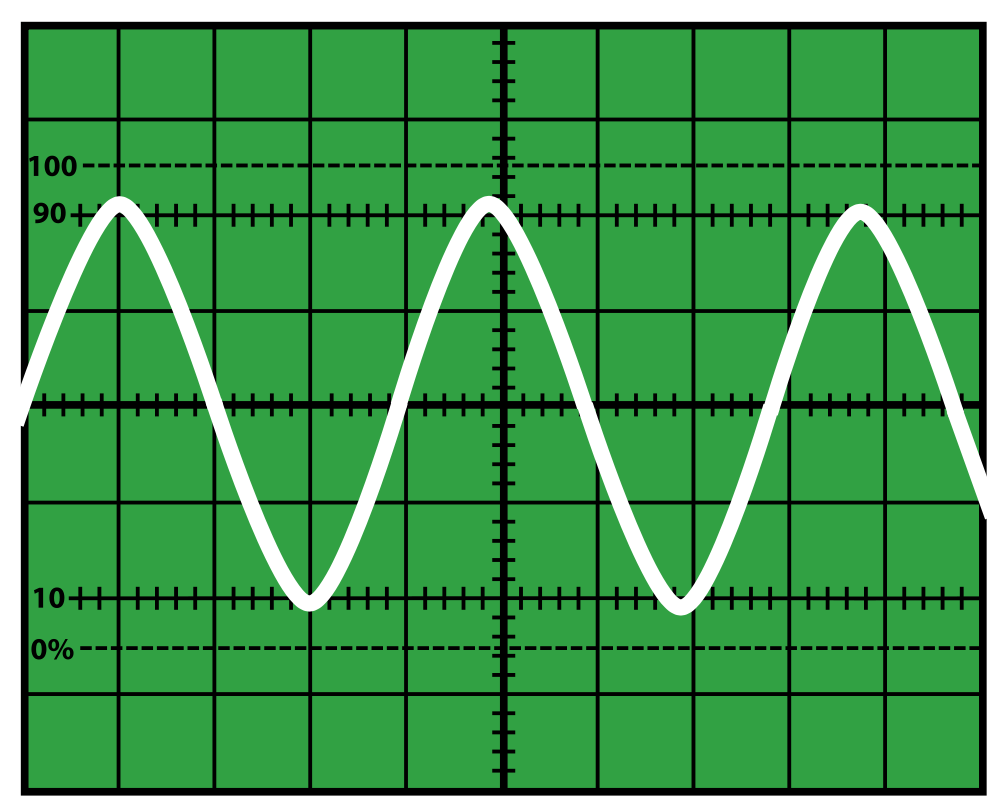
\includegraphics[width=.8\textwidth,height=.7\textheight,keepaspectratio]{e17/OsziTon.png}
        \footnote{\tiny \url{https://commons.wikimedia.org/wiki/File:Oszi_Ton.svg}}
	\end{center}
\end{frame}

\begin{frame}
    \frametitle{Spannungen}
    \begin{center}
    \begin{itemize}
			\item PEP -- Peak to Peak
			\item RMS -- Effektivwert
			\item $u_{Spitze} = \sqrt{2} \cdot U_{eff}$ \\
    \end{itemize}
  \end{center}
  \begin{exampleblock}{Aufgabe}
    Berechnet Spitzen-Spitzen Spannung vom Netzstrom
  \end{exampleblock}
\end{frame}

\section*{Dipmeter}

\begin{frame}
    \frametitle{Dipmeter}
    \begin{center}
        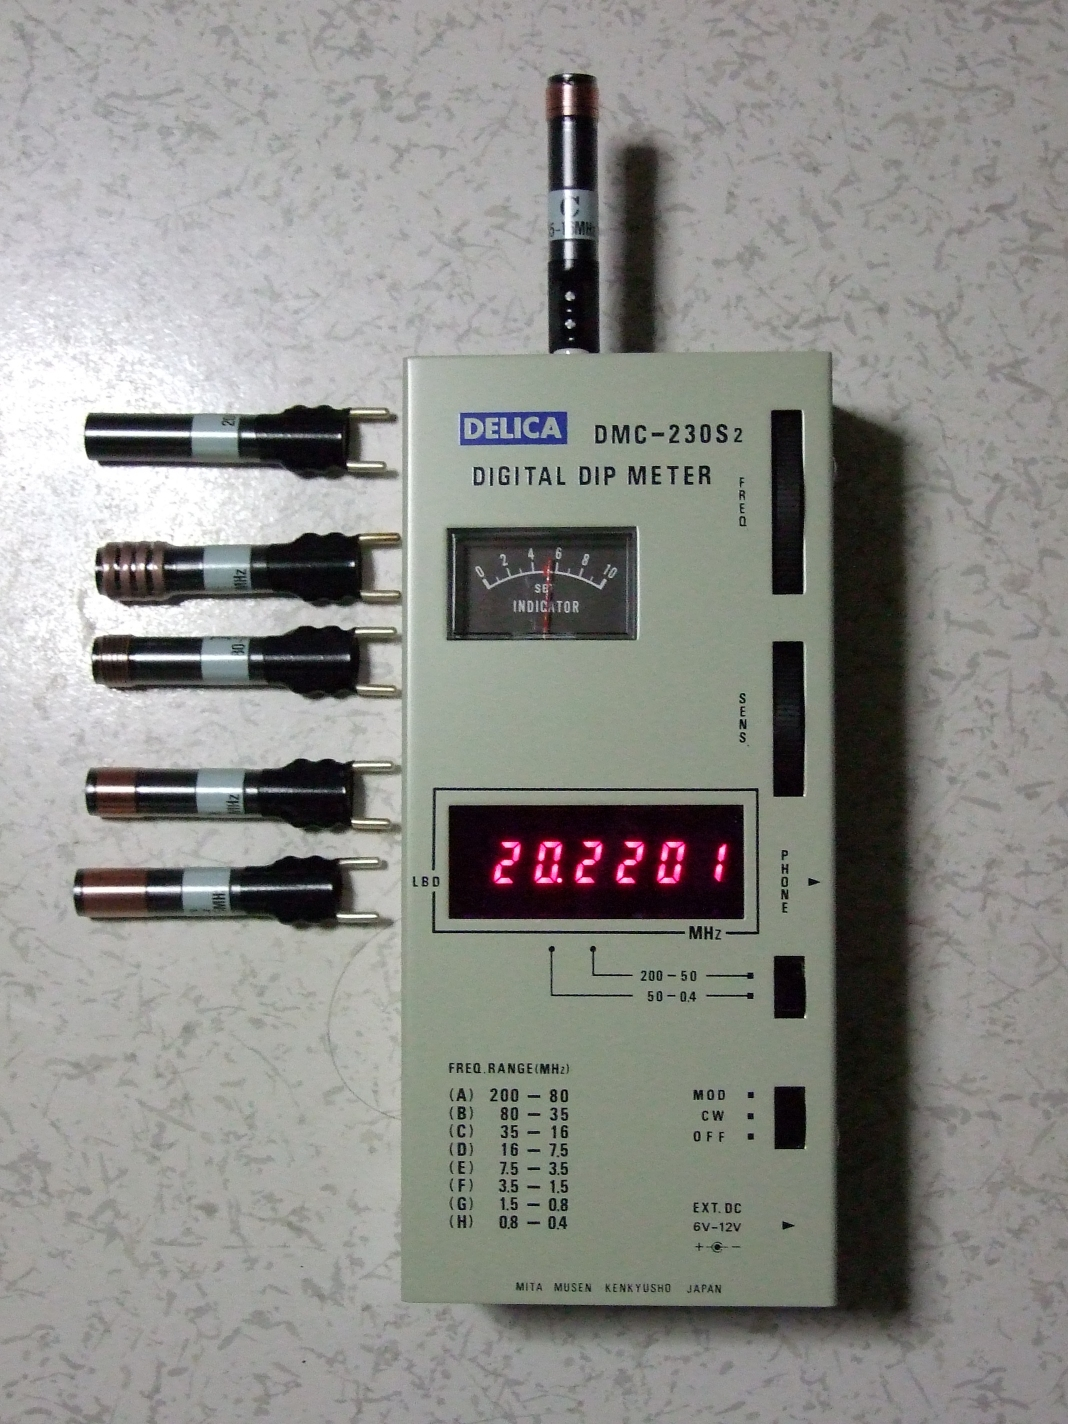
\includegraphics[width=0.55\textwidth,height=.8\textheight,keepaspectratio]{e17/Dipmeter.jpg}
        \footnote{\tiny \url{https://commons.wikimedia.org/wiki/File:Dipmeter_and_its_probe_coils.jpg}}
	\end{center}
\end{frame}

\section*{SWR-Meter}

\begin{frame}
    \frametitle{Stehwellenmessgerät}
    \begin{center}
        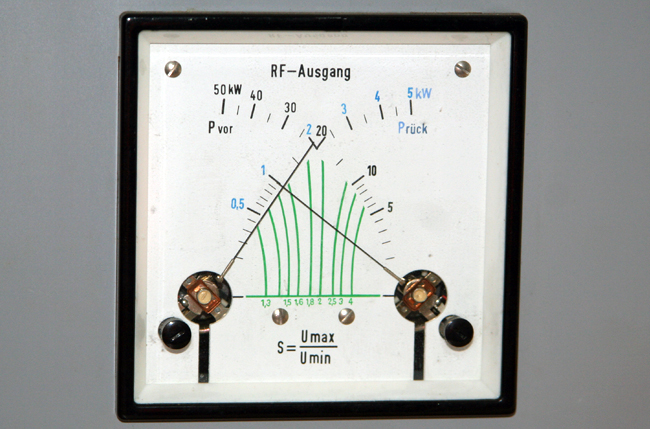
\includegraphics[width=1\textwidth,height=.8\textheight,keepaspectratio]{e17/RS_SWR.jpg}
        \footnote{\tiny \url{https://commons.wikimedia.org/wiki/File:RS_SWR.jpg}}
	\end{center}
\end{frame}

\begin{frame}
    \frametitle{Interner Aufbau}
    \begin{block}{S-Wert Berechnung}
      $$s = \cfrac{U_{max}}{U_{min}} = \cfrac{U_v + U_r}{U_v - U_r}$$
    \end{block}
    \begin{center}
      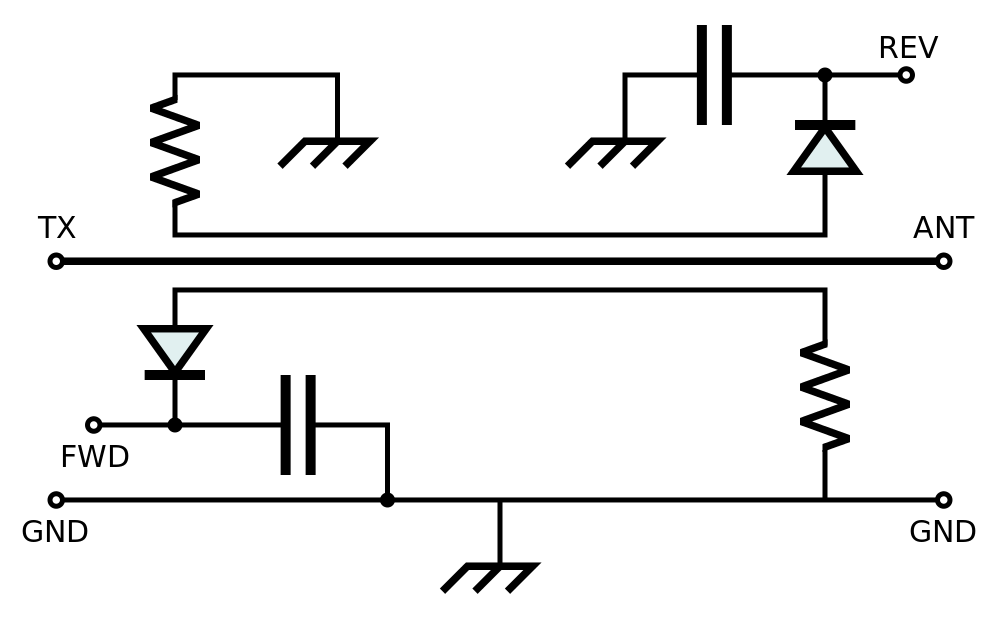
\includegraphics[width=.8\textwidth,height=.5\textheight,keepaspectratio]{e17/SWRMeterInnen.png}
      \footnote{\tiny \url{https://commons.wikimedia.org/wiki/File:SWR_Meter.svg}}
    \end{center}
\end{frame}

\begin{frame}
    \frametitle{VSWR-Rechnen}
    \begin{exampleblock}{Beispiel}
      \begin{center}
	$$s = \frac{U_{max}}{U_{min}} = \frac{U_v + U_r}{U_v - U_r}$$
	$$s = \frac{1V + 0.5V}{1V - 0.5V} = \frac{1.5V}{0.5V} = 3$$
	$$s = \frac{1V + 0V}{1V - 0V} = \frac{1V}{1V} = 1$$
      \end{center}
    \end{exampleblock}
\end{frame}


\begin{frame}
    \frametitle{Prüfungsfrage}
    \begin{center}
      \begin{tabular}{l||p{.8\textwidth}}\hline
	\textbf{TH401} & \textbf{Eine Antenne hat ein Stehwellenverhältnis (VSWR) von 3. Wie viel Prozent der Sendeleistung wird von der Antenne abgestrahlt, wenn sonst keine Verluste auftreten?}\\ \hline\hline
         A & $50 \%$ \\\hline
         B & $29 \%$ \\\hline
         C & $25 \%$ \\ \hline
         D \only<2>\checkmark & $75 \%$\\\hline
    \end{tabular}\\[1.5em]
    \only<2>{$50 \%$ der Spannung sind $25 \%$ der Leistung.}
 	\end{center}
\end{frame}

\begin{frame}
    \frametitle{Wo das SWR-Meter einschleifen?}
    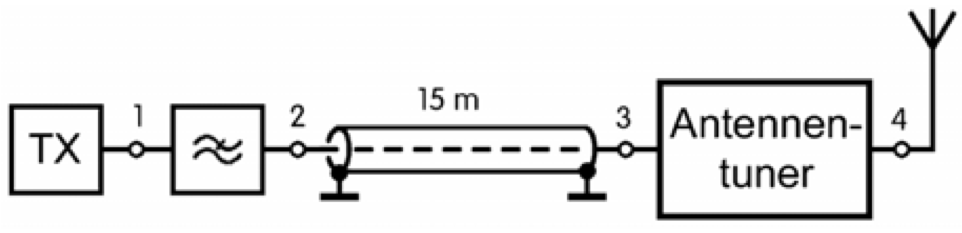
\includegraphics[width=.97\textwidth,height=.4\textheight,keepaspectratio]{e17/SWROrt.png}
    \footnote{\tiny Fragenkatalog BundesNetzAgentur Klasse E}
    \pause
    Am Besten in 1, da alles dahinter zur Antenne bzw. Antennenanlage gehört.
\end{frame}


\section*{Dummy Load}

\begin{frame}
    \frametitle{Messen}
    \begin{center}
        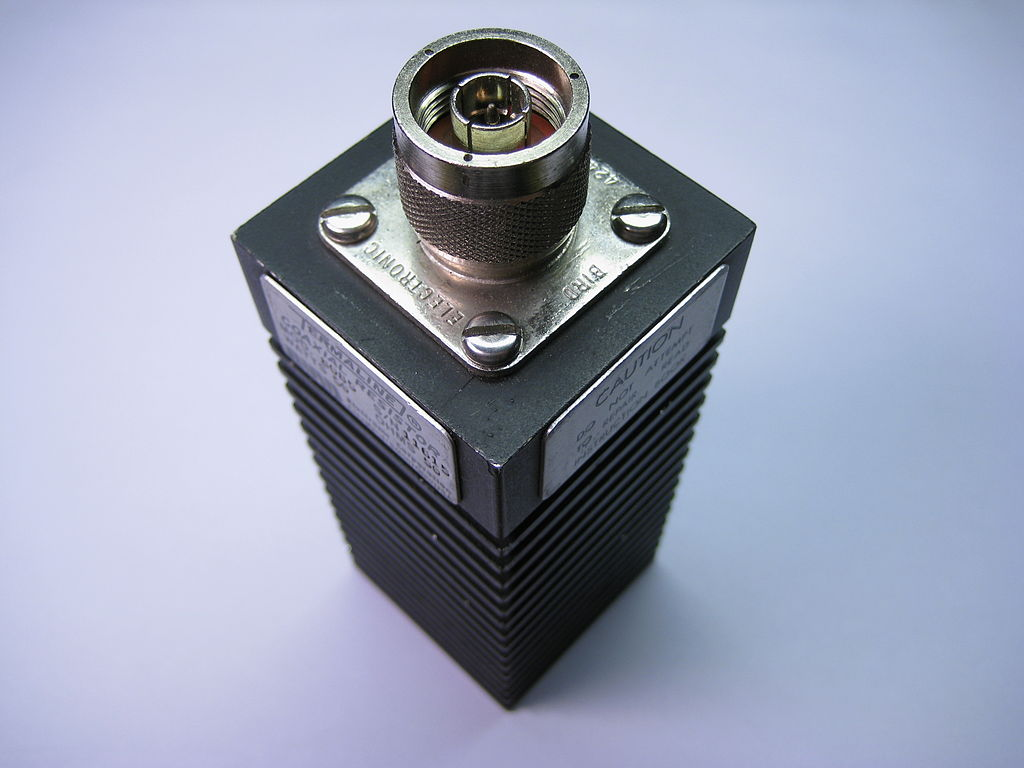
\includegraphics[width=.99\textwidth,height=.8\textheight,keepaspectratio]{e17/DummyLoad.jpg}
        \footnote{\tiny \url{https://commons.wikimedia.org/wiki/File:Dummy_load.jpg}}
	\end{center}
\end{frame}

\begin{frame}
    \frametitle{Zu Beachten}
    \begin{itemize}
		\item Aufbau als Widerstandsdekade
		\item Genau $50 \Omega$ Realer Widerstand
		\item Lastwiderstände
		\item Am besten Metalloxid-Widerstände
		\item Große Kühlkörper
		\item Selbstbau: \url{http://der-bastelbunker.blogspot.de/2011/04/qro-dummy-load-von-kw-bis-vhf-fur-1.html}
    \end{itemize}
\end{frame}

\begin{frame}
    \frametitle{Dummyload in der Sendeanlage Nauen}
	\begin{minipage}{0.4\textwidth}
	\begin{center}
	    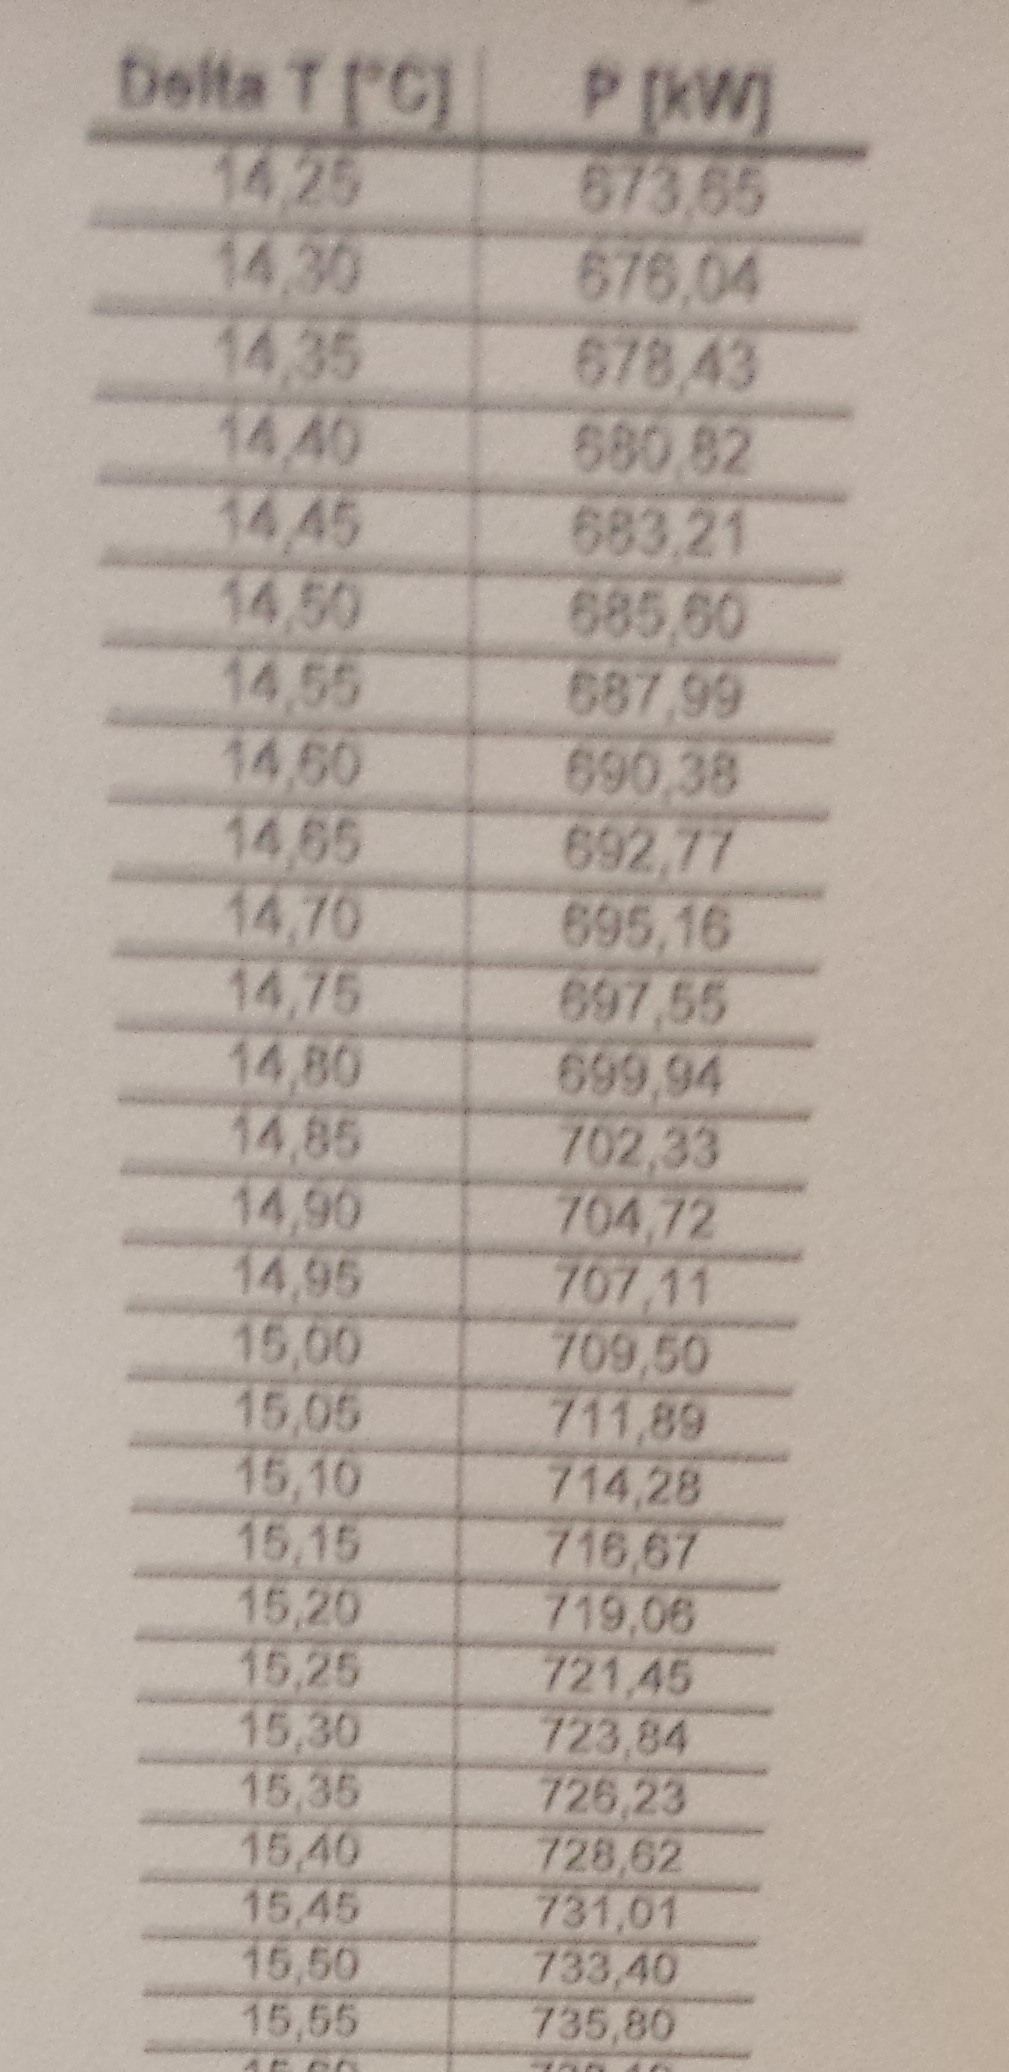
\includegraphics[width=.9\textwidth,height=.8\textheight,keepaspectratio]{e17/DummyNauen.jpg}
	\end{center}
	\end{minipage}
	        \footnote{\tiny Bild DB4UM}
		%\hspace{0.5cm}
	\begin{minipage}{0.55\textwidth}
	\begin{itemize}
		\item Dummyload in Nauen
		\item Auch als Wattmeter nutzbar
		\item Temperaturanstieg pro Zeiteinheit
	\end{itemize}
	\end{minipage}
\end{frame}

\section*{Referenzen}

\begin{frame}
    \frametitle{Referenzen/Links}
    
    \footnotesize
    \begin{itemize}
        \item Moltrecht E 17: \\
              \url{http://www.darc.de/referate/ajw/ausbildung/darc-online-lehrgang/technik-klasse-e/technik-e17/}
         \item SWR-Meter Selbstbau \\
         	\url{http://www.nogaqrp.org/projects/NOGAwatt/nogawattwithnewschematic2.pdf}
         \item Dummy Selbstbau \\
         	\url{http://der-bastelbunker.blogspot.de/2011/04/qro-dummy-load-von-kw-bis-vhf-fur-1.html}
    \end{itemize}

\end{frame}

% Hier könnte noch eine Kontaktfolie stehen

\end{document}

